\subsection{$n$D-Sphere-line picking}
\label{sec:nsphere_line}

Sphere-line picking is subtly different from ball-line picking. In
this new case, we choose points on the surface of a 2-sphere (the
sphere in 3D), but the lines are straight lines in the 3D space in
which the sphere is embedded, i.e., we use the standard Euclidean
distance metric.

$n$-Sphere is embedded in $\R^{n+1}$ and encloses the $n+1$-ball

The $2$-sphere is the set of points $S^n = \big\{ {\mathbf x} \in \R^2
\; \big| \; \|{\mathbf x} \|_2 \leq R \big\},$ where $R$ is the {\em
  radius}.
% http://en.wikipedia.org/wiki/N-sphere

Figure~\ref{fig:sphere_eg} shows an example of the line-picking
problem on the 2-sphere. Generating points uniformly on the sphere
requires a little care: it can be accomplished by taking
\cite{marsaglia72:_choos_point_surfac_spher}
\begin{equation}
    \label{eq:x_surface_sphere2}
    \x = R \frac{\y}{\| \y \|_2}, 
\end{equation}
where the $y_i \sim N(0,1)$ are IID standard normal random variates.
The result is a set of points chosen so that the probability of there
being $k$ points inside non-overlapping regions of are $a$ takes
IID Poisson distributions with mean $\lambda a$ where $\lambda =
m/V_n$, where $m$ is the total number of points generated, and $S_2$
is the surface area of the sphere.

\begin{figure}[tbp]
  \begin{center}
    \subfloat[\label{fig:sphere_eg}2-sphere example.]
       {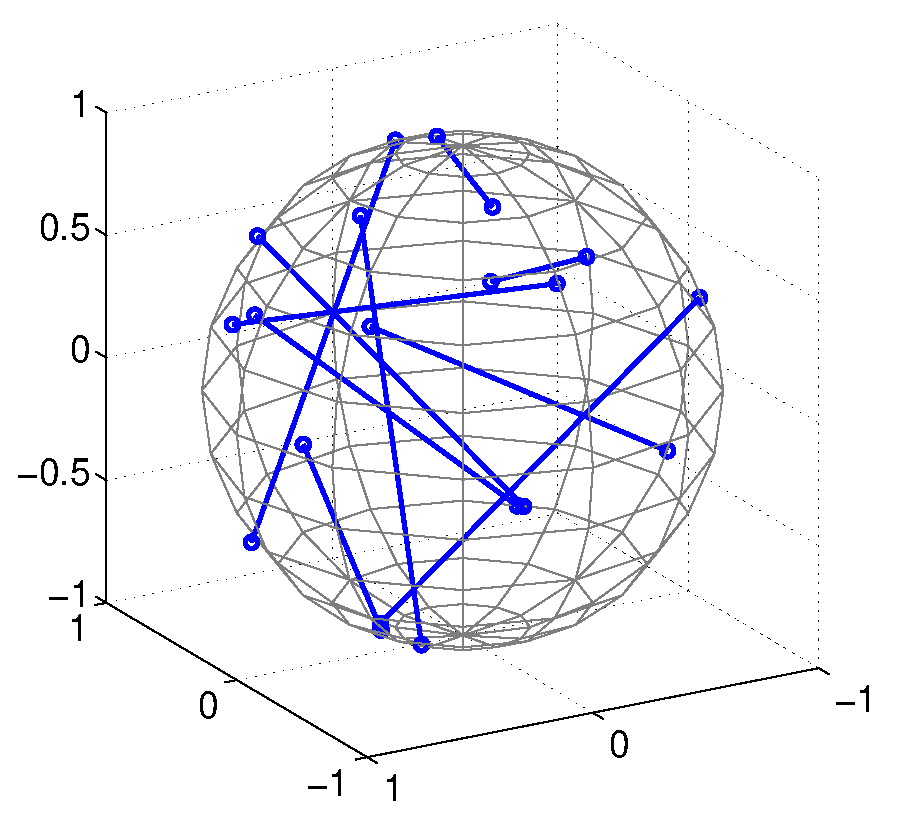
\includegraphics[width=0.4\columnwidth]{../Matlab/Plots/LinePicking_eg_sphere.eps}} 
    \hspace{6mm}
    \subfloat[\label{fig:sphere_pdf}PDF of $n$-spheres.]
       {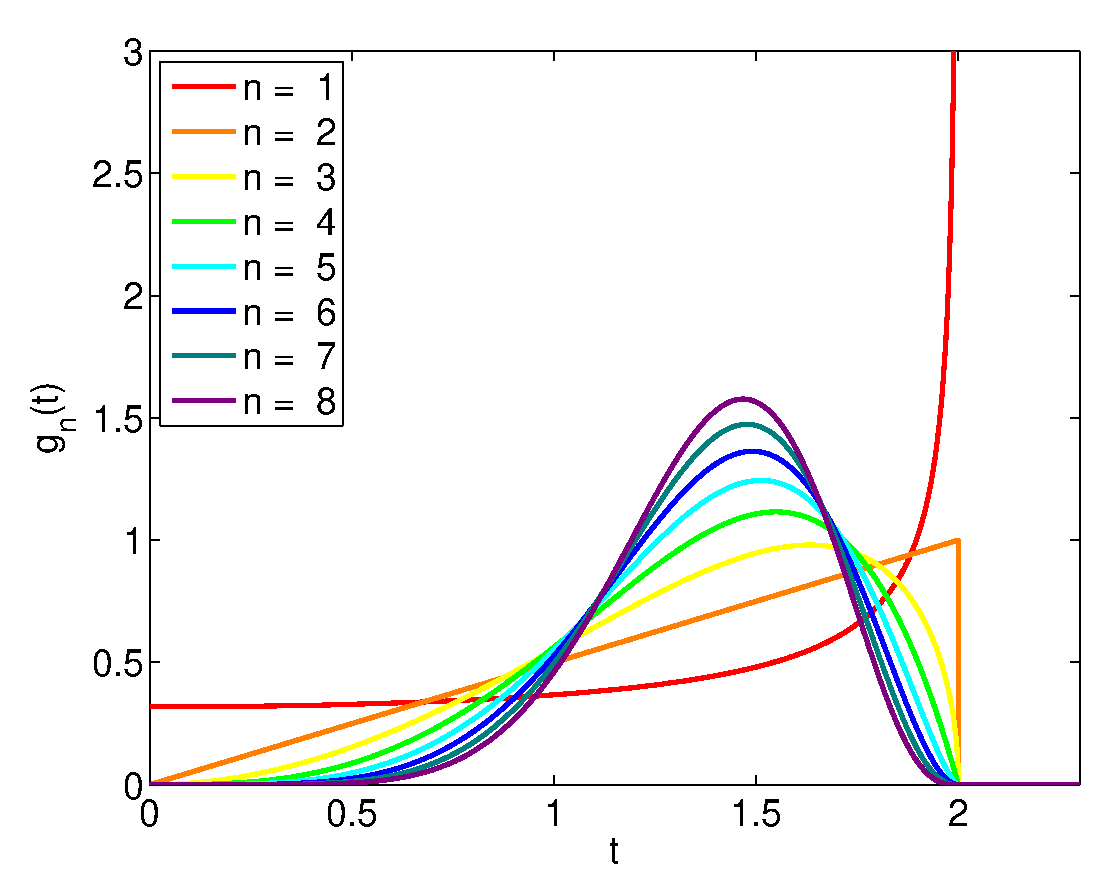
\includegraphics[width=0.48\columnwidth]{../Matlab/Plots/LinePicking_plot_nspheres.eps}}
    \caption{The $n$-sphere-line picking problem.}
  \end{center} 
\vspace{-4mm}
\end{figure}

\subsubsection{PDF}

Obviously, the sphere has spherical symmetry, but as a result, we can,
without loss of generality, assume the first point lies at the pole of
the sphere.

Points on the $n$-sphere can be parameterised by a set of angles
$\phi_1, \phi_2, \ldots, \phi_{n-1}$ where $\phi_1, \phi_2, \ldots,
\phi_{n-2}\in [0,\pi]$ and $\phi_{n-1}\in [0,2\pi)$. 


We can transform to Cartesian coordinates of $\R^{n+1}$ by
\begin{eqnarray}
  \label{eq:sphere_to_cart1}
  x_1 & = & R \cos (\phi_1 ) \\
  x_2 & = & R \sin(\phi_1) \cos (\phi_2 ) \\
  x_3 & = & R \sin(\phi_1) \sin(\phi_2) \cos (\phi_3 ) \\
      & \vdots & \\
  x_{n} & = & R \sin (\phi_1) \sin(\phi_2) \cdots \sin (\phi_{n-1}) \cos (\phi_{n})  \\
  x_{n+1} & = & R \sin (\phi_1) \sin(\phi_2) \cdots \sin (\phi_{n-1}) \sin (\phi_{n}) 
  \label{eq:sphere_to_cartn}
\end{eqnarray}

So the first point is chosen at the pole where
$\phi_1=\phi_2=\cdots=\phi_{n-1}=0$, so that ${\mathbf x} =
(R,0,0,\ldots,0)$, and the second point satisfies equations
\eqref{eq:sphere_to_cart1}-\eqref{eq:sphere_to_cartn}. 

Distance is therefore
\begin{eqnarray}
  \label{eq:d_nsphere}
  d^2 & = & R^2 \left[ 
                        (1-\cos(\phi_1))^2
                       + \sin^2 (\phi_1) \cos^2 (\phi_2 )
                       + \sin^2 (\phi_1) \sin^2 (\phi_2) \cos^2 (\phi_3 )
                       + \cdots \right.  \nonumber \\
     & &   \left.           + \sin^2 (\phi_1) \sin^2 (\phi_2) \cdots \sin^2 (\phi_{n-1}) \cos^2 (\phi_{n})
                       + \sin^2 (\phi_1) \sin^2 (\phi_2) \cdots \sin^2 (\phi_{n-1}) \sin^2 (\phi_{n}) 
                 \right].
\end{eqnarray}
The last two terms sum, using $\cos^2 (\phi_{n}) + \sin^2
(\phi_{n}) = 1$, and then the resulting last two terms sum
likewise, and so on collapsing the whole sum down to
\begin{eqnarray}
  \label{eq:d_nsphere}
  t^2 & = & R^2 \left[ 
                        (1-\cos(\phi_1))^2
                       + \sin^2 (\phi_1) \right], \nonumber \\
 & = & R^2 \left[ 1 - 2 \cos(\phi_1) + \cos^2(\phi_1)
                       + \sin^2 (\phi_1) \right], \nonumber \\
 & = & 2 R^2 \left[ 1 - \cos(\phi_1) \right].
\end{eqnarray}
So distance only depends on the first (angular) coordinate.


Uniformly chosen at random means that in any (generalized) area
element of size $t^{n}S$, there will be, on average $\lambda t^{n}S$
points (where $\lambda$ is the rate of points, which is simply the
total number of points divided by the total (generalized) area).

A small area unit on the $n$-sphere can be written (in terms of the
Jacobian $J$)
\begin{eqnarray}
  \label{eq:vn_n_sphere}
  t^nS & = & J \, d\phi_1 \, d\phi_2 \, \cdots d\phi_{n},  \nonumber \\
       & = & \sin^{n-1}(\phi_1) \sin^{n-2}(\phi_2) \cdots \sin(\phi_{n-1})
                  d\phi_1 \, d\phi_2 \, \cdots d\phi_{n}.
\end{eqnarray}
To obtain the distribution for distances, we integrate the distance
function over these elements to obtain the density of the first
angular coordinate, i.e.,
\begin{eqnarray}
  f(\phi_1)
      & = & \sin^{n-1}(\phi_1)
              \int_{0}^{2\pi} \int_{0}^{\pi} \cdots  \int_{0}^{\pi} 
              \sin^{n-2}(\phi_2) \cdots \sin(\phi_{n-1})
                   d\phi_2 \, \cdots d\phi_{n}, \nonumber \\
      & = & \sin^{n-1}(\phi_1)
              \int_{0}^{2\pi} 1 d\phi_{n} 
              \int_{0}^{\pi} \sin(\phi_{n-1}) d\phi_{n-1}  
              \cdots  
              \int_{0}^{\pi} \sin^{n-2}(\phi_2)  d\phi_{2}, \nonumber \\   
\end{eqnarray}
From \cite[3.621,5.(p.369)]{GandR}, the integral
\begin{equation}
  \int_0^{\pi/2} \sin^{n-1}(x) \, dx
     = \frac{1}{2} B\left( n/2, 1/2 \right)
     = \frac{1}{2} \frac{\Gamma(n/2) \Gamma(1/2)}{\Gamma((n+1)/2)},   
\end{equation}
or 
\begin{equation}
  \label{eq:int_sin_n}
  \int_0^{\pi} \sin^{n-1}(x) \, dx = 
       \frac{\sqrt{\pi} \, \Gamma\big( n/2 \big)}{\Gamma\big( (n+1)/2 \big)}.
\end{equation}
Note that in each adjacent term in the product above, the Gamma
functions in the numerators and denominators cancel so the final
product collapses down to
\begin{eqnarray}
  f(\phi_1)
      & = & \sin^{n-1}(\phi_1)
              \int_{0}^{2\pi} 1 d\phi_{n} 
              \int_{0}^{\pi} \sin(\phi_{n-1}) d\phi_{n-1}  
              \cdots  
              \int_{0}^{\pi} \sin^{n-2}(\phi_2)  d\phi_{2}, \nonumber \\   
      & = & 2 \pi \pi^{(n-2)/2} \sin^{n-1}(\phi_1)  
                     \frac{\Gamma\big( 1 \big)}{\Gamma\big( n/2 \big)}
                 \nonumber \\   
      & = &  \frac{4 \pi^{n/2}}{\Gamma\big( n/2 \big)} \sin^{n-1}(\phi_1)  .
\end{eqnarray}
which we can see from \eqref{eq:int_sin_n} must result in
\begin{equation}  
 g(\phi) = \frac{\Gamma\left(\frac{1+n}{2}\right)}
                  {\sqrt{\pi } \Gamma\left(\frac{n}{2}\right)} 
                      \sin(\phi )^{n - 1}.
\end{equation} 
We have have a function for $t$ the distance between two points in
terms of $\phi_1$ so we can get  $\phi_1$ in terms of $t$ thus: 
\begin{eqnarray}
  t^2 & = & 2 R^2 \left[ 1 - \cos(\phi_1) \right].\\
\phi_1& =  & \cos^{-1} \left[1-\frac{t^2}{2 R^2}\right]\\ 
   \frac {d \phi_1}{dt} & = &\frac{t}{\sqrt{1-\left(1-\frac{t^2}{2 R^2}\right)^2} R^2} \\
   & = &\frac{2}{\sqrt{4 R^2 -t^2 }}.
\end{eqnarray}
If $y = g(X)$ then the transform rule  is :  
\[ f_Y(y) = \left| \frac{d}{dy} \left( g^{-1}(y) \right) \right|
                f_X\left( g^{-1}(y) \right).
\]

Thus we can write:
\begin{eqnarray}
  g^{n-{\rm sphere}}_{n,R}(t)
    & = & \left|\frac{2}{\sqrt{4 R^2 -t^2 }} \right|
             g_{\Phi}\left( \cos^{-1} \left[1-\frac{t^2}{2  R^2}\right]\right) \nonumber \\
    & = & \frac{t \left(\frac{t^2}{R^2} -\frac{t^4}{4 R^4}\right)^{\frac{1}{2} (n-2)}
             \Gamma\left[\frac{1+n}{2}\right]}{\sqrt{\pi } R^2 \Gamma\left[\frac{n}{2}\right]}  \nonumber \\
    & = & \frac{t \left(\frac{t}{R} \right)^{(n-2)}
             \left(1 -\frac{t^2}{4 R^2}\right)^{\frac{1}{2} (n-2)}
             \Gamma\left[\frac{1+n}{2}\right]}{\sqrt{\pi } R^2 \Gamma\left[\frac{n}{2}\right]}  \nonumber \\
    & = & \frac{2^{n-1} \left(\frac{t}{2R} \right)^{n-1}
             \left(1 -\frac{t^2}{4 R^2}\right)^{\frac{1}{2} (n-2)}
             \Gamma\left[\frac{1+n}{2}\right]}{\sqrt{\pi } R \Gamma\left[\frac{n}{2}\right]}  
\end{eqnarray}
using the fact that $\sin\big( \cos^{-1}(x) \big) = \sqrt{1 - x^2}$.
Now using the Gauss multiplication formula: 
\begin{equation}
(2\pi)^{((m-1)/2)}m^{(1/2-mz)} \Gamma\left[mz\right]=\Sigma_{k=0}^{m-1}\Gamma\left[z+\frac{k}{m}\right].  \nonumber \\ 
\end{equation}
which for $m = 2$ and $z = n/2$ gives
\begin{equation}
 2^{-(n-1)}\sqrt{ \pi } \Gamma\left[n\right]=\Gamma\left[\frac{n+1}{2}\right] \Gamma\left[\frac{n}{2}\right].  
  \label{eq:gamma_rel}
\end{equation}
so we get
\begin{eqnarray}
  g^{n-{\rm sphere}}_{n,R}(t)
    & = & \frac{\left(\frac{t}{2R} \right)^{n-1}
             \left(1 -\frac{t^2}{4 R^2}\right)^{\frac{1}{2} (n-2)}\Gamma\left[n\right]}
             { R \Gamma\left[\frac{n}{2}\right]^2}.
  \label{eq:nsphere_pdf_phi}
\end{eqnarray}


The obvious special cases are the circle (the 1-sphere) and the 2-sphere where the
above becomes:
\begin{eqnarray}
  g^{n-{\rm sphere}}_{1,R}(t) 
   & = &\frac{\left(1 -\frac{t^2}{4 R^2}\right)^{-\frac{1}{2}}}{\pi R}, \\
  g^{n-{\rm sphere}}_{2,R}(t) 
   & = &\frac{t}{2 R^2}.
\end{eqnarray}

The PDF for the 2-sphere is unusual in that it, and the line-line
picking problem CDFs are exactly opposite (and these are the only two
that have their mode at one end of the support, i.e., these are the
only two monotonic densities.



\subsubsection{CDF}

The cumulative density function is derived by integrating the PDF:
\begin{eqnarray}
G^{n-{\rm sphere}}_{n,R}(t)
       & = & \int_0^t g^{n-{\rm sphere}}_{n,R}(s) \, ds \nonumber \\
       & = & \frac{ \left(1-\frac{s^2}{4 R^2}\right)^{-n/2} 
                    \left( \frac{s^2}{R^2} \right)
                   -\frac{s^4}{4 R^4})^{n/2} 
                    \Gamma \left[\frac{1+n}{2}\right] {}_{2}F_{1} 
                    \left[ 1-\frac{n}{2},\frac{n}{2},1+\frac{n}{2},\frac{s^2}{4 R^2} \right]
                  }{n \sqrt{\pi } \Gamma \left[ \frac{n}{2} \right] }.
\end{eqnarray}
This can be simplified a little further using a regularised
Hypergeometric function rather than the general one above :
\begin{equation}
G^{n-{\rm sphere}}_{n,R}(t) = 
      \frac{\left(\frac{t^2}{R^2} -\frac{t^4}{4 R^4}\right)^{n/2}
            \Gamma\left[\frac{1+n}{2}\right]
             {}_{2}\bar{F}_{1}\left[1,n,\frac{2+n}{2},\frac{t^2}{4
                 R^2}\right]
           }{2 \sqrt{\pi }}.
\end{equation}


     
A better alternate derivation: take $u={\left(\frac{s}{2R}\right)}^2$, so $s = 2R \sqrt{u}$ and $ds = du\; R / \sqrt{u}$ then
\begin{eqnarray}
G^{n-{\rm sphere}}_{n,R}(t)
    & = & \int_0^t g^{n-{\rm sphere}}_{n,R}(s) \, ds \nonumber \\
    & = & \int_0^t  2^{n-1} \frac{\left( \frac{s}{2R}\right) {\left({\left( \frac{s}{2R}\right)}^{2}\right)}^{\frac{n}{2} -1}
             {\left(1 - {\left( \frac{s}{2R}\right)}^{2}  \right)}^{\frac{n}{2} -1}
             \Gamma\left[\frac{1+n}{2}\right]}{R\sqrt{\pi }
             \Gamma\left[\frac{n}{2}\right]} 
             \, ds, \nonumber \\    
    & = & \frac{ 2^{n- 1} \Gamma\left[\frac{1+n}{2}\right]}{R\sqrt{\pi}\Gamma\left[\frac{n}{2}\right]}
           \int_0^t \left( \frac{s}{2R}\right) {\left({\left( \frac{s}{2R}\right)}^{2}\right)}^{\frac{n}{2} -1}
             {\left(1 - {\left( \frac{s}{2R}\right)}^{2}  \right)}^{\frac{n}{2} -1}
             \, ds, \nonumber \\    
    & = & \frac{ 2^{n-1} \Gamma\left[\frac{1+n}{2}\right]}{R\sqrt{\pi}\Gamma\left[\frac{n}{2}\right]}
           \int_0^{ {\left(\frac{t}{2R}\right)}^{2} } u^{(n-1)/2}  \left(1 - u\right)^{\frac{1}{2} (n-2)}
             \, du R / \sqrt{u}  \nonumber \\    
    & = & \frac{ 2^{n-1} \Gamma\left[\frac{1+n}{2}\right]}{\sqrt{\pi}\Gamma\left[\frac{n}{2}\right]}
           \int_0^{{\left(\frac{t}{2R}\right)}^{2}} u^{n/2-1}  \left(1 - u\right)^{n/2-1)}
             \, du,  \nonumber \\    
    & = & \frac{ 2^{n-1} \Gamma\left[\frac{1+n}{2}\right]}{\sqrt{\pi}\Gamma\left[\frac{n}{2}\right]}
               \beta_{{\left(\frac{t}{2R}\right)}^{2}}(n/2, n/2),  \nonumber \\    
    & = & \frac{ 2^{n-1} \Gamma\left[\frac{1+n}{2}\right] \Gamma\left[\frac{n}{2}\right] }{\sqrt{\pi}\Gamma\left[\frac{n}{2}\right]^2}
               \beta_{{\left(\frac{t}{2R}\right)}^{2}}(n/2, n/2),  \nonumber \\ 
\end{eqnarray}


Now using the Gauss multiplication formula: 
\begin{equation}
(2\pi)^{((m-1)/2)}m^{(1/2-mz)} \Gamma\left[mz\right]=\Sigma_{k=0}^{m-1}\Gamma\left[z+\frac{k}{m}\right].  \nonumber \\ 
\end{equation}
which for $m = 2$ and $z = n/2$ gives
\begin{equation}
 2^{-(n-1)}\sqrt{ \pi } \Gamma\left[n\right]=\Gamma\left[\frac{n+1}{2}\right] \Gamma\left[\frac{n}{2}\right].   \nonumber \\ 
\end{equation}

Thus:
\begin{eqnarray}
G^{n-{\rm sphere}}_{n,R}(t)
    & = &\frac{\Gamma \left[n \right] {\beta}_{{\left(\frac{t}{2 R}\right)}^{2}}\left( \frac{n}{2},\frac{n}{2}\right)}
     {\Gamma\left[\frac{n}{2}\right]^{2}},  \nonumber \\   
     & = &  {I}_{{\left(\frac{t}{2 R}\right)}^{2}}\left( \frac{n}{2},\frac{n}{2}\right).
\end{eqnarray}




Alt derivation: for $R=1/2$, and taking $u=s^2$, so $s = \sqrt{u}$ and
$ds = du/2\sqrt{u}$
\begin{eqnarray}
G^{n-{\rm sphere}}_{n,1/2}(t)
    & = & \int_0^t g^{n-{\rm sphere}}_{n,1/2}(s) \, ds \nonumber \\
    & = & \int_0^t  2^n \frac{s^{n-1}
             \left(1 -s^2\right)^{\frac{1}{2} (n-2)}
             \Gamma\left[\frac{1+n}{2}\right]}{\sqrt{\pi }
             \Gamma\left[\frac{n}{2}\right]} 
             \, ds \nonumber \\    
    & = & \frac{ 2^n \Gamma\left[\frac{1+n}{2}\right]}{\sqrt{\pi}\Gamma\left[\frac{n}{2}\right]}
           \int_0^t s^{n-1}  \left(1 -s^2\right)^{\frac{1}{2} (n-2)}
             \, ds \nonumber \\    
    & = & \frac{ 2^n \Gamma\left[\frac{1+n}{2}\right]}{\sqrt{\pi}\Gamma\left[\frac{n}{2}\right]}
           \int_0^{t^2} u^{(n-1)/2}  \left(1 - u\right)^{\frac{1}{2} (n-2)}
             \, du/2\sqrt{u}  \nonumber \\    
    & = & \frac{ 2^{n-1} \Gamma\left[\frac{1+n}{2}\right]}{\sqrt{\pi}\Gamma\left[\frac{n}{2}\right]}
           \int_0^{t^2} u^{n/2-1}  \left(1 - u\right)^{n/2-1)}
             \, du  \nonumber \\    
    & = & \frac{ 2^{n-1} \Gamma\left[\frac{1+n}{2}\right]}{\sqrt{\pi}\Gamma\left[\frac{n}{2}\right]}
               \beta_{t^2}(n/2, n/2)  \nonumber \\    
    & = & \frac{ 2^{n-1} \Gamma\left[\frac{1+n}{2}\right]}{\sqrt{\pi}\Gamma\left[\frac{n}{2}\right]}
              \beta(n/2,n/2) I_{t^2}(n/2, n/2)  \nonumber \\    
    & = & \frac{ 2^{n-1} \Gamma\left[\frac{1+n}{2}\right]}{\sqrt{\pi}\Gamma\left[\frac{n}{2}\right]}
              \frac{\Gamma[n/2]^2}{\Gamma[n]} I_{t^2}(n/2, n/2)  \nonumber \\    
    & = & \frac{ 2^{n-1} \Gamma\left[\frac{1+n}{2}\right]\Gamma[n/2] }{\sqrt{\pi}\Gamma\left[n\right]}
              I_{t^2}(n/2, n/2)  \nonumber \\    
\end{eqnarray}




\subsubsection{Moments}


If $y = g(X)$

\[ f_Y(y) = \left| \frac{d}{dy} \left( g^{-1}(y) \right) \right|
               f_X\left( g^{-1}(y) \right)
\]


\begin{eqnarray}
 E[ g(X) ] & = & \int y f_g (y) \, dy  \nonumber \\
           & = & \int g(x) f_X(x) \, dx  \nonumber \\
           & = &  \frac{n^{2}  R  {\Gamma\left[ \frac{1 + n}{2} \right]}^{2} }{ \sqrt{\pi} \Gamma\left[ n + \frac{1}{2} \right]  }            
\end{eqnarray}


Taking $R=1/2$, we get $k$th moment is
\begin{eqnarray}
E[ X^k ] 
    & = & \int_0^1 s^k g^{n-{\rm sphere}}_{n,1/2}(s) \, ds \nonumber \\
    & = & \frac{\Gamma\left[n\right]}{R \Gamma\left[\frac{n}{2}\right]^2} 
          \int_0^1 s^k s^{n-1}  \left(1 - s^2\right)^{\frac{1}{2} (n-2)}
               \, ds \nonumber \\
    & = & \frac{\Gamma\left[n\right]}{2 R \Gamma\left[\frac{n}{2}\right]^2} 
          \int_0^1 u^{(k+n)/2-1}  \left(1 - u \right)^{n/2-1}
               \, du \nonumber \\
    & = & \frac{\Gamma\left[n\right] B\big( (k+n)/2,n/2 \big)}
               {2 R \Gamma\left[\frac{n}{2}\right]^2}  \nonumber \\
    & = & \frac{\Gamma\left[ n \right] \Gamma\left[ (k+n)/2 \right]}
               {2 R \Gamma\left[\frac{n}{2}\right] \Gamma\left[ n+k/2 \right] } 
          \nonumber 
\end{eqnarray}
To obtain the general case for $R$, we multiply by $(2R)^k$ to get
\begin{eqnarray}
E[ X^k ] 
    & = & \frac{(2R)^{k-1} \Gamma\left[ n \right] \Gamma\left[ (k+n)/2 \right]}
               {\Gamma\left[\frac{n}{2}\right] \Gamma\left[ n+k/2 \right] } 
\end{eqnarray}
